\section{Abbreviations}

\begin{itemize}
    \item \textbf{FOV}: Field of View
    \item \textbf{HST}: Hubble Space Telescope
    \item \textbf{JWST}: James Webb Space Telescope
    \item \textbf{OTA}: Optical Telescope Assembly
    \item \textbf{OTE}: Optical Telescope Element
    \item \textbf{ACS}: Advanced Camera for Surveys
    \item \textbf{WFC3}: Wide Field Camera 3
    \item \textbf{STIS}: Space Telescope Imaging Spectrograph
    \item \textbf{COS}: Cosmic Origin Spectrograph
    \item \textbf{FGS}: Fine Guidance Sensors
    \item \textbf{MIRI}: Mid Infra-Red Instrument
    \item \textbf{NIRCam}: Near Infra-Red Camera
    \item \textbf{NIRISS}: Near Infrared Imager and Slitless Spectrograph
    \item \textbf{NIRSpec}: Near Infra-Red Spectrograph
\end{itemize}

\section{Introduction}

Both Hubble and James Webb space telescopes use the vacuum of space to avoid atmospheric visual interference that a ground telescope would suffer from.

The Hubble space telescope was launched into low Earth orbit in 1990 and so far has completed 35 years of service with several repairs, last done in 2009 and expected to last until 2030 at least and 2040 in the best outcome.

The James Webb space telescope was launched into the Sun-Earth L2 orbit in 2021 and started its mission in 2023. It is meant as an upgrade over the Hubble telescope and is expected to survive at least 20 years, up to 2043. A comparison in the observation image quality can be found in figure \ref{fig:comparing_jwst_hst}. 

Both telescopes use mirror-based optical telescope assemblies that share some common design ideas, such as the basics of Cassegrain design, which uses large primary mirrors to collect large amounts of incoming light and through a system of mirrors (reflective, correction, pick-off) redirect it onto a comparatively small observation sensors. These detectors are usually either CCD (note in \ref{thm:ccd}), MAMA (note in \ref{thm:mama}) or HgCdTe (note in \ref{thm:hgcdte}). 

\clearpage
\section{Hubble Optic System}

The HST is a Ritchey-Chrétien Cassegrain type telescope capable of observing/recording light in the range of $100$ to $2500nm$ with a maximum surface error of $10nm$ ($\frac{1}{65}$ of the bottom edge of visible light). This range gives the HST the ability to work in visible, near-ultraviolet, and infrared spectrums, which is reflected in the equipment that HST uses for observations. The main observation instruments that the HST uses are:

\begin{itemize}
    \item Advanced Camera for Surveys (ACS, 2002)
    \item Wide Field Camera 3 (WFC3, 2009)
    \item Space Telescope Imaging Spectrograph (STIS)
    \item Cosmic Origins Spectrograph (COS)
    \item Fine Guidance Sensors (FGS)
\end{itemize}

These instruments can be broken down into two categories: cameras and spectrometers.

\subsection{Optical Telescope Assembly}
\label{subsec:hst_ota}

As mentioned above, the HST uses a Ritchey-Chrétien Cassegrain telescope type, which uses a two mirror setup. The primary mirror collects light and reflects it towards a secondary mirror in front of the primary mirror that reflects the light down through a hole in the primary mirror towards the instruments. The assembly can be seen in figure \ref{fig:hst_optical_telescope_assembly}.

\begin{table}[h]
    \centering
    \begin{tabular}{cccc}
        \textbf{Diameter} & \textbf{Focal Length} & \textbf{f-ration} & \textbf{Area} \\
        $2.4m$ & $57.6$ & $24$ & $4.0m^2$ \\
    \end{tabular}
    \caption{HST OTA Information \cite{hubble_optics_simpson_2010}}
    \label{tab:hst_ota_information}
\end{table}

The OTA is a static mirror setup with no built-in fine-motion control. Any adjustments in the observations are done through either the current position/rotation of the telescope or the instruments themselves.

\begin{figure}[h]
    \centering
    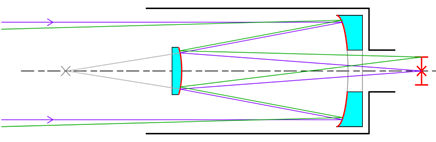
\includegraphics[width=0.9\linewidth]{images/hst_ota.png}
    \caption{HST: Optical Telescope Assembly Diagram}
    \label{fig:hst_optical_telescope_assembly}
\end{figure}

\subsection{Advanced Camera for Surveys}

The ACS is the third generation (older) camera instrument currently on board, being installed in 2002 and serviced only partially since. It contains two main optical paths and three main detectors with a specific sensor, resolutions, and FOV information contained in table \ref{tab:ACS_channel_information}. 

The first path is the Wide Field Channel that uses a CCD sensors and is used for imaging in visible to near-IR light. The second path contains two separate sensors, the Solar Blind Channel detector and the High Resolution Channel detector. The HRC like the WFC used a CCD sensor, but with different resolutions and FOV, but unfortunately this channel is currently non-functional and it will most probably remain this way.

\begin{Note}{CCD Detector}{fermat}
    \label{thm:ccd}
    A charge-coupled device uses a a photoactive area and a 2D array of linked capacitors to capture images. These capacitors are linked in columns and form shift registers. All shift registers are connected to another perpendicular shift register. 
    
    Capturing an image through a CCD sensor is done through exposing the photoactive region, which accumulates charge in each position within the vertical shift registers. These shift registers are subsequently read in series (row-by-row) through the horizontal shift register. All of the registers shift by one each time a row is read, which introduces some transmission issues. 
\end{Note}

The SBC uses a Multi-Anode Microchannel Array (MAMA) with the same resulution as HRC, but different FOV. 

\begin{Note}{MAMA Detector}{fermat}
    \label{thm:mama}
    A Multi-Anode Microchannel Array, commonly referred to as MAMA, is a photon-counting detector array that is used in ground and space telescopes for high-sensitivity, high-resolution, photometrically stable imaging \cite{4331264} in near-UV light.
\end{Note}

Both optical paths contain systems of filters. The first system contains two filter wheels (each wheel contains filters on its edge, and rotating them selects the filter) and is shared between the WFC and HRC sensors. The shared filter system allowed for simultaneous observations on both sensors under specific filter combinations. The second system is only for the SBC sensor and contains only one wheel.

\subsection{Wide Field Camera 3}

The Wide Field Camera 3 (WFC3) is a fourth generation instrument. It contains two main optical paths and sensors, which have a shared pickup from the incoming OTA light through a 45° mirror. A flat channel select mirror can then be inserted into the light to direct the light into one of the paths (channels). Similar specifications as for the ACS instruments can be found in table \ref{tab:wfc3_channel_information}.

The first path is the UV/vis channel (UVIS) and is used in a way similar to the ACS/WFC for observations in the visible to near-IR light and also uses the same type and nearly same size of CCD sensors.

The second path is the near-infrared channel (IR), which uses a special compound of mercury cadmium telluride (HgCdTe) for its infrared detector. Both optical paths can be seen in figure \ref{fig:wfc3_optical_system_overview}, where blue represents the UVIS and red the IR.

\begin{figure}[h]
    \centering
    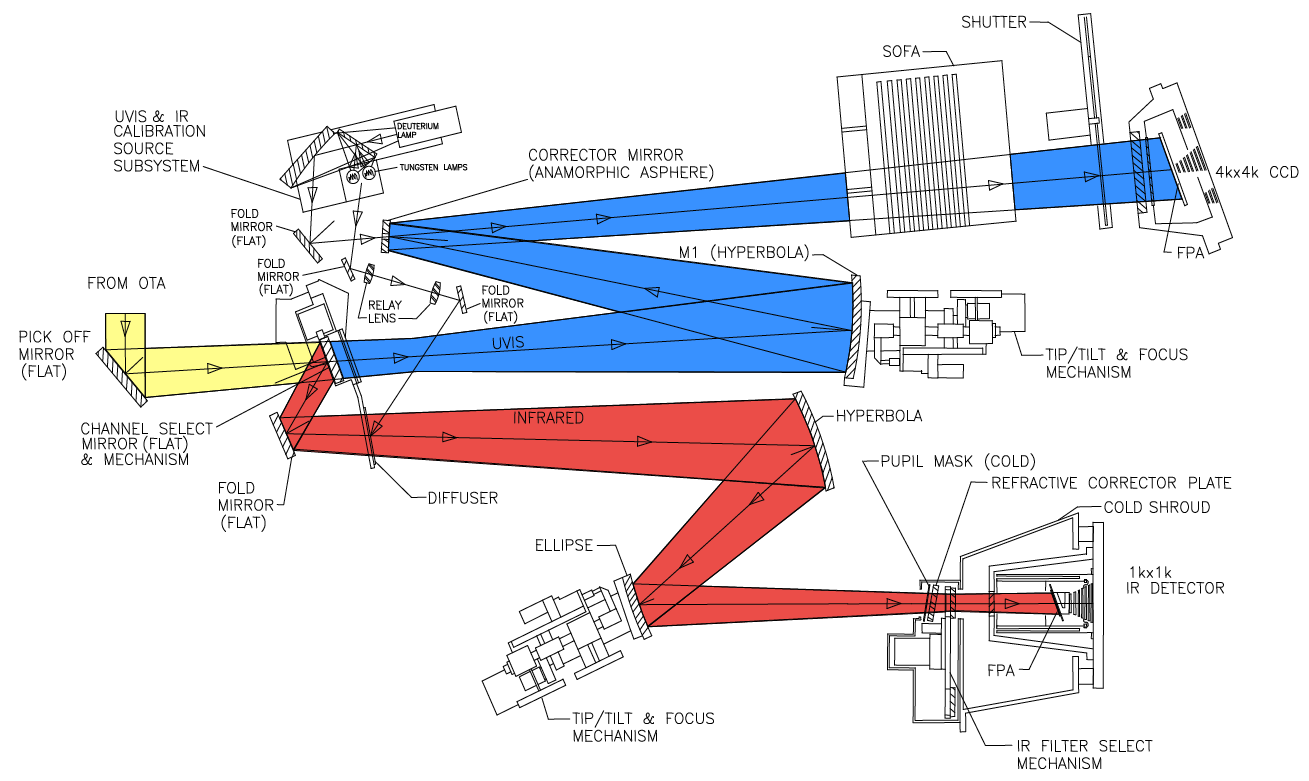
\includegraphics[width=0.95\linewidth]{images/wfc3_optical_system.png}
    \caption{WFC3: Optical System Overview}
    \label{fig:wfc3_optical_system_overview}
\end{figure}

\begin{Note}{HgCdTe Detector}{fermat}
    \label{thm:hgcdte}
    HgCdTe detectors use a composite material is a special mixture of CdTe (semiconductor) and HgTe (semimetal) that is sensitive to infrared light at very low temperatures (145K).
\end{Note}

\subsection{Space Telescope Imaging Spectrograph}

The STIS has been a versatile spectrograph on board since 1997 with many functionalities complementary to the COS \cite{HST_STIS}. 

STIS contains three types of detectors, CCD and two MAMAs, each having $1024\times 1024$ resolution. The selection of which detector is done through camera mirrors, mode selection wheel, and slit wheel. These modes can do many functions, such as imaging, spectroscope (slit and slitless), coronagraphy, etc.

\subsection{Cosmic Origins Spectrograph}

The complement to STIS, the COS was installed into the HST in 2009 and is a far-ultraviolet spectrograph designed to observe large structures within the universe, which filled the HST capabilities, as there were no such UV spectroscopes on board before \cite{HST_COS}.

COS contains two main pathways: far-ultraviolet and near-ultraviolet, where only one channel can be observed at a time. COS is essentially a slit-less spectrograph that has a very small FOV. 

The incoming light is first sent through one of several selectable apertures, which is followed by optical selection mechanics (OSM1). This mechanics can select from four options: a flat mirror that reflects the light towards the NUV path, and the rest are gratings for the FUV path. The FUV path directly ends after this step on a detector, while the NUV path continues through more mirrors and a second optics selection mechanics (OSM2), before also landing on a detector. Both paths can be seen in figure \ref{fig:hst_cos_diagram}.

\begin{figure}[h]
    \centering
    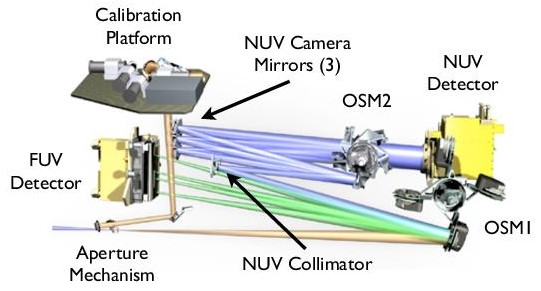
\includegraphics[width=0.9\linewidth]{images/hst_cos_diagram.jpg}
    \caption{HST: COS Diagram}
    \label{fig:hst_cos_diagram}
\end{figure}

\subsection{Fine Guidance Sensors}

The last notable instrument on board of the HST are the FGS. These sensors are large FOV interferometers capable of tracking luminous points with an extremely high precision of around $~1$ milli-arc-second (mas). Additionally, the FGS can scan an object to obtain its interferogram \cite{HST_FGS}.

The optical path of each FGS contains three primary elements: Star Selector A, Start Selector B, and Interferometer Assembly. The SSA and SSB are mirror based assemblies that can be commanded to rotate the telescopes optical axis. Between the star selectors and the interferometers is a flat filter wheel. The interferometer assembly contains two paths, divided by a polarising beam splitter. Each path further splits the incoming light through a Koester prism (prisms rotated $90°$). All light paths go through focusing optics onto photomultiplier tube detectors. This entire FGS assembly can be seen in figure \ref{fig:hst_fgs_diagram}.

\begin{figure}[h]
    \centering
    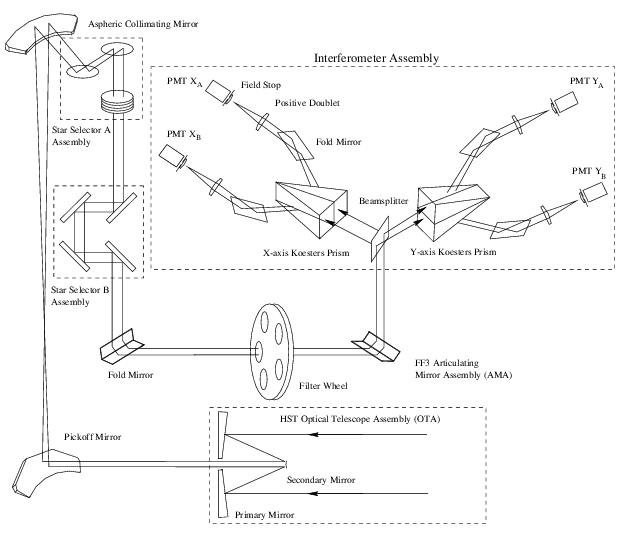
\includegraphics[width=0.9\linewidth]{images/hst_fgs_diagram.jpg}
    \caption{HST: FGS Diagram}
    \label{fig:hst_fgs_diagram}
\end{figure}

\subsection{Initial Optical Issues}

Amongst the many discoveries towards which the HST contributed, one of the most known situations regarding its life is an initial flaw in its optics. Two months after launching in 1990, NASA has announced that there is a flaw within the optics affecting the instruments on-board.

The issue was a presence of spherical abberation that could only happen on either the primary or secondary mirror as all instruments were affected, meaning it was not an issue in them. An investigation of the optical manufacturing found that the primary mirror had a wrong curve (too flat on the edges). The error was nearly 10 times higher than the tolerance allowed (around $1.2mm$) and was created during manufacturing due to an incorrect setup of the testing device called the \textit{null detector}.

The spherical aberration created an issue in which the light picked up from the primary mirror had several focal points instead of one as was designed. This resulted in the output images being blurry as the light from one source was spread across the surrounding area. This can be described by a \textit{point spread function} (PSF), which was extracted from the HST through observation of a single point light, creating an impulse response. The resulting image of the single star was blurred in the same way as the PSF, which can be seen in figure \ref{fig:hst_constar_comparison}.

\begin{figure}[h]
    \centering
    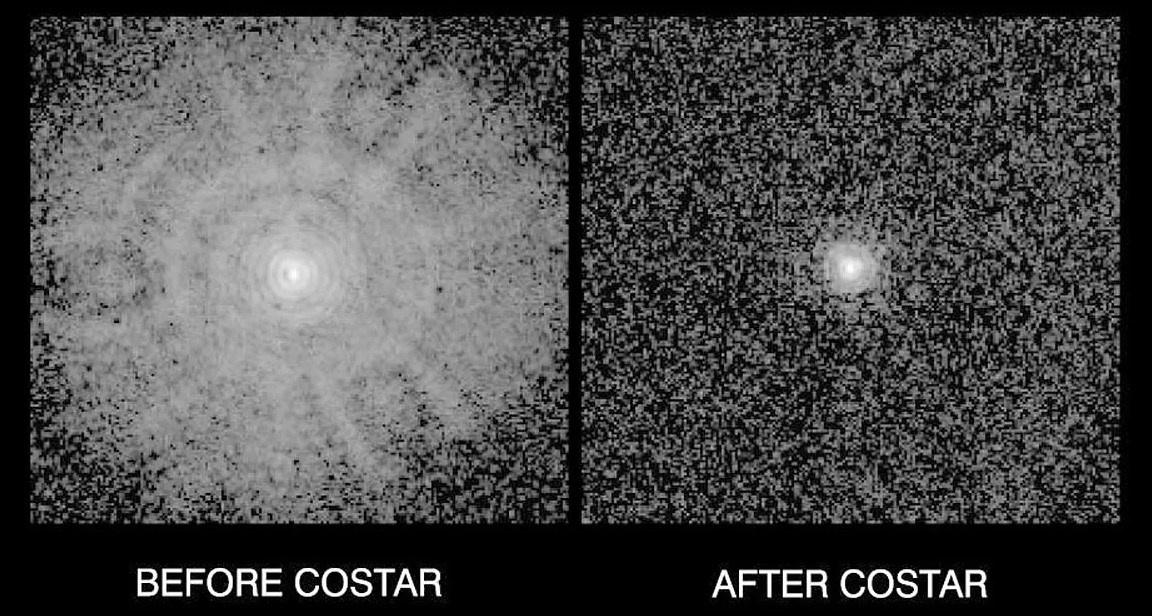
\includegraphics[width=0.9\linewidth]{images/hst_constar_fix.jpg}
    \caption{HST: CONSTAR Comparison}
    \label{fig:hst_constar_comparison}
\end{figure}

With the extracted PSF, the teams working on the telescope were able to develop Hubble’s Corrective Optics Space Telescope Axial Replacement (CONSTAR), which was a package installed onto HST during the first servicing mission in 1993. In plain words, CONSTAR were glasses for the HST, which mitigated the spherical aberration issue. The before and after can be seen again in figure \ref{fig:hst_constar_comparison}.

Each instrument installed later already contained corrective optics within their light paths, and in 2009, during the fourth service mission, the CONSTAR was removed and replaced by COS \cite{HST_Optical_Fault}. 

\begin{table*}
    \centering
    \small
    \begin{tabular}{ccccccc}
        \textbf{Channel} & \textbf{f-ratio} & \textbf{Sensor Type} & \textbf{Spectral Range (nm)} & \textbf{Pixel Format} & \textbf{Pixel Scale (arcsec)} & \textbf{FOV (arcsec)}\\
        WFC & $30$ & CCD & $350-1100$ & $2 \times 2048 \times 4096$ & $\sim 0.5\times 0.5$ & $202 \times 202$ \\
        HRC & $72$ & CCD & $170-1100$ & $1014 \times 1014$ & $\sim 0.028 \times 0.025$ & $29\times 26$ \\
        SBC & $72$ & MAMA & $115-170$ & $1014 \times 1014$ & $\sim 0.034 \times 0.030$ & $34.6 \times 30.5$\\
    \end{tabular}
    \caption{ACS: Channel Information \cite{HST_ACS}}
    \label{tab:ACS_channel_information}
\end{table*}

\begin{table*}
    \centering
    \small
    \begin{tabular}{ccccccc}
        \textbf{Channel} & \textbf{f-ratio} & \textbf{Sensor Type} & \textbf{Spectral Range (nm)} & \textbf{Pixel Format} & \textbf{Pixel Scale (arcsec)} & \textbf{FOV (arcsec)}\\
        UVIS & $31$ & CCD & $200-1000$ & $2 \times 2051 \times 4096$ & $\sim 0.04 \times 0.04$ & $162 \times 162$ \\
        IR & $11$ & HgCdTe & $800-1700$ & $1014 \times 1014$ & $\sim 0.13 \times 0.13$ & $136 \times 123$ \\
    \end{tabular}
    \caption{WFC3: Channel Information \cite{HST_WFC3}}
    \label{tab:wfc3_channel_information}
\end{table*}

\section{James Webb Optic System}

As mentioned in the introduction, the James Webb Space Telescope (JWST) is orbiting within Earth's L2 orbit, which is within the special group of orbits that use the Lagrange points (thus L1-5 orbits) that have special properties unlike normal low-orbit, geostationary, etc. orbits. When a lighter object orbits a heavier object (the Earth and the Sun here) and we would plot a line through their centres of mass, then the second Lagrange point is upon this line, outside the interval between the two objects and on the smaller objects side (Earth's) in such a distance that the combined gravitational forces upon an object in this point would make the object stationary from the point of view of the line\cite{JWST_Orbit}.

In other words, it is a special orbit that is going to be locked in place in relation to earth and the Sun, which the JWST uses to its advantage in many ways. For example, temperature control, where the instruments onboard (both OTE and ISIM) require rather low temperatures to operate correctly, and this locked orbit helps mitigate issues that would arise from, for example, geo-stationary orbit. This is combined with the sun shield skirts attached at the midsection of the telescope (the bottom is always facing the sun), which further isolates the observation section from any sunlight and from any infra-red light that the telescope itself emits. This achieves an operating temperature of 40-50 K on the instrument side and 300 K on the side facing the sun \cite{JWST_Observatory_Article}. These skirts can be seen in the figure \ref{fig:jwst_top_view}.

\begin{figure}[h]
    \centering
    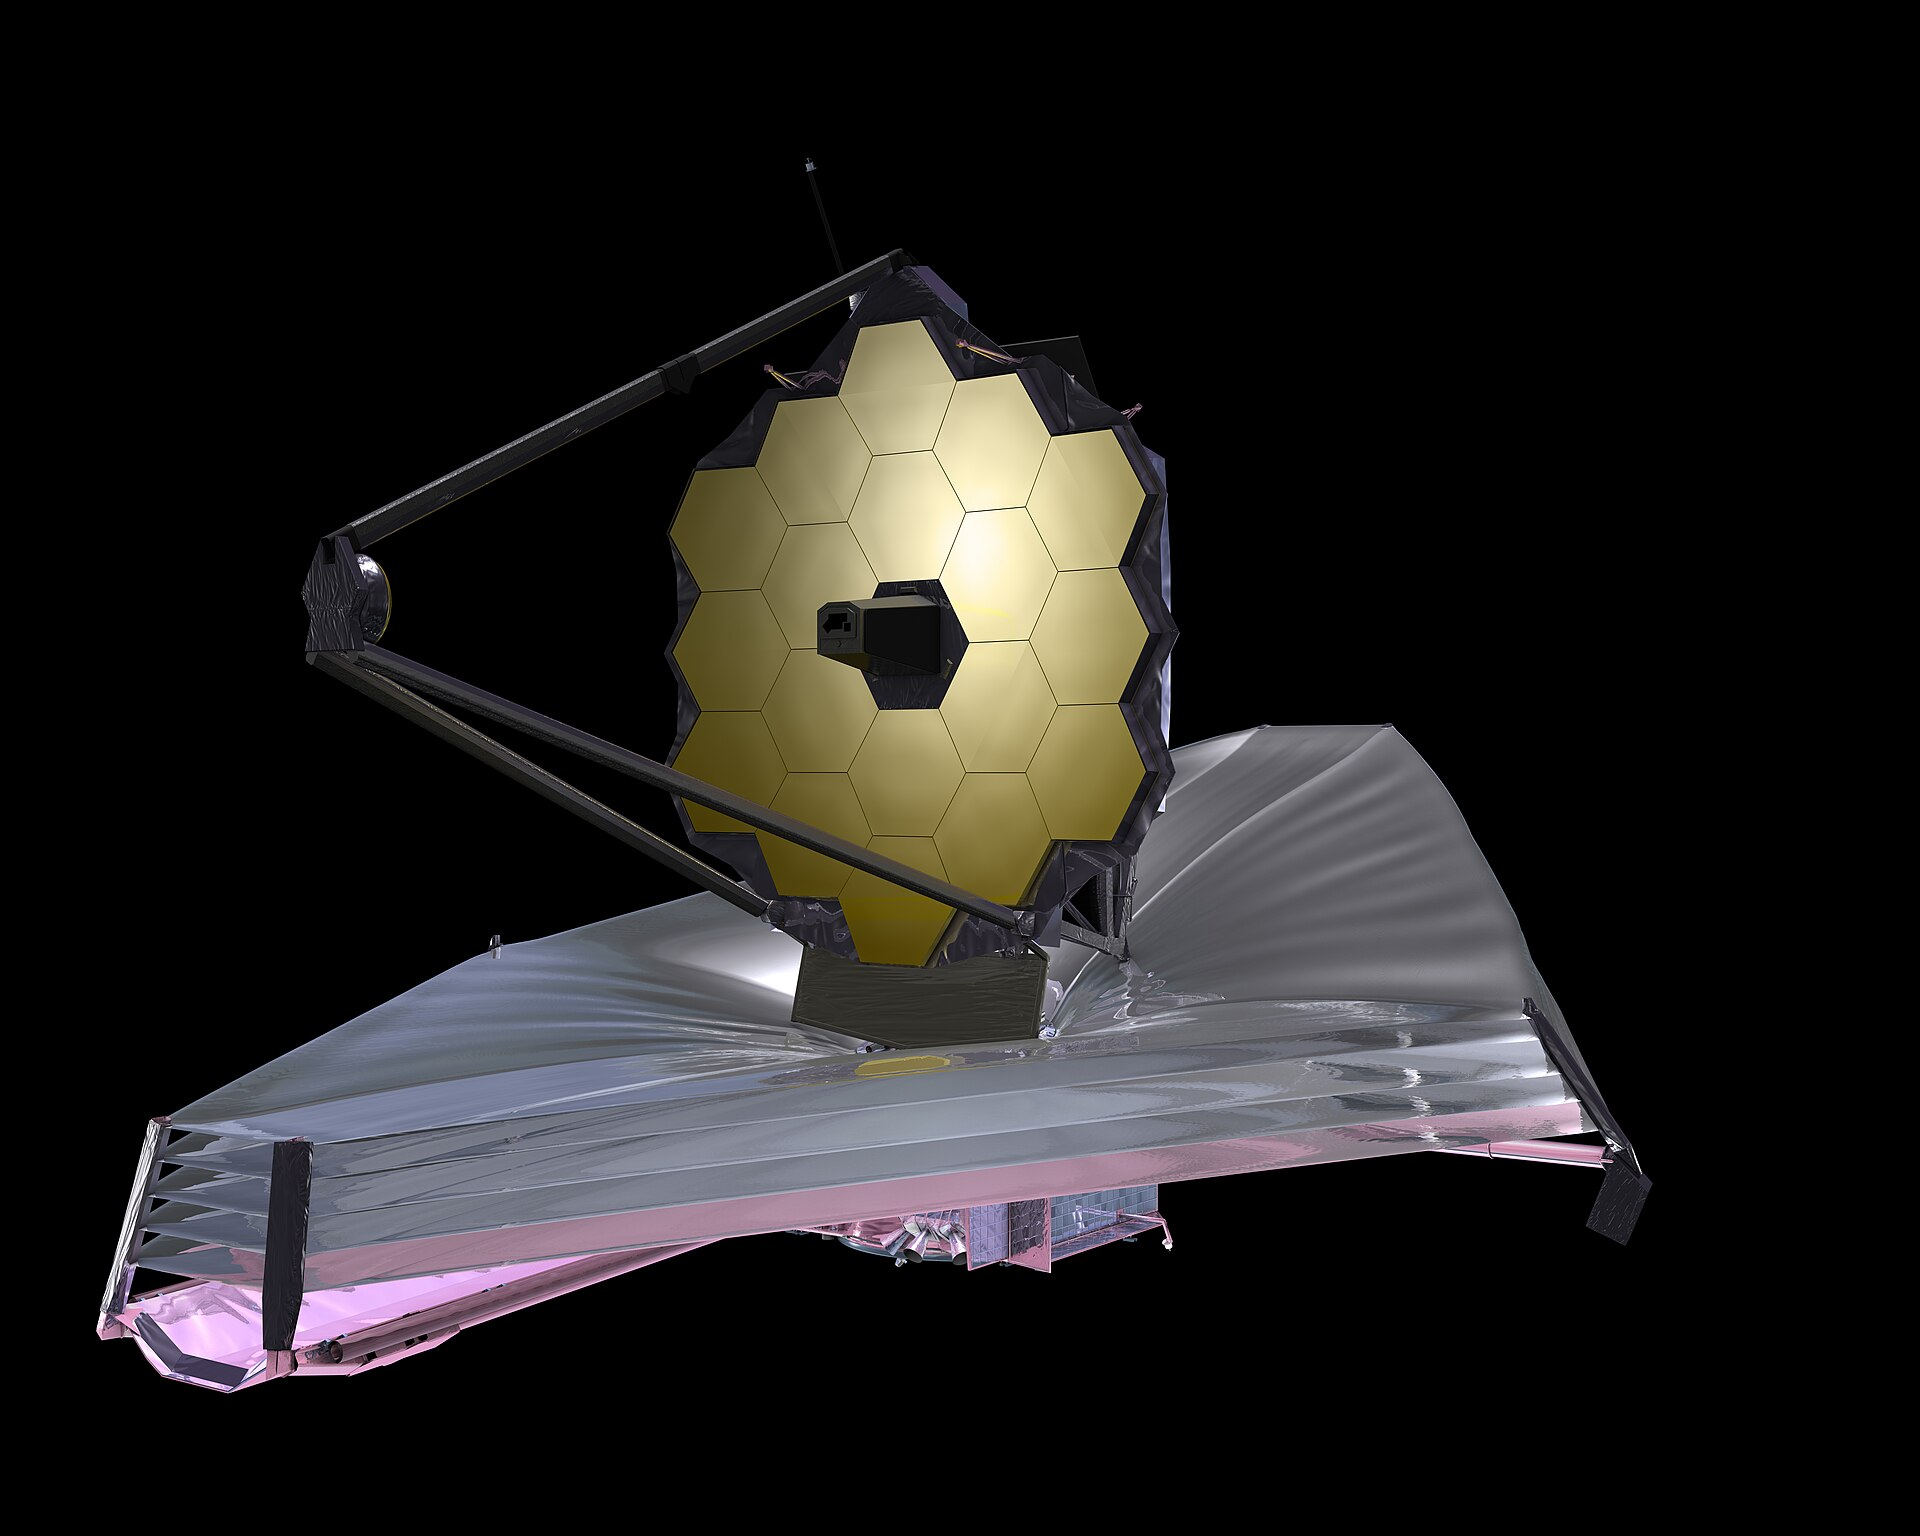
\includegraphics[width=0.9\linewidth]{images/1920px-James_Webb_Space_Telescope_2009_top.jpg}
    \caption{JWST: Top View with sun skirts and mirrors visible.}
    \label{fig:jwst_top_view}
\end{figure}

The JWST is divided into several sections, but in this project the only relevant parts are the \textit{Optical Telescope Element} (OTE) and the \textit{Integrated Science Instrument Module} (ISIM).

\subsection{Optical Telescope Element}

The OTE was created using the \textbf{3-mirror anastigmat} design, which uses 4 mirrors to gather light. It uses a primary mirror, secondary mirror, tertiary mirror, and a fourth flat mirror called the \textbf{fine steering mirror} (FSM), which is the only adjustable mirror used for stabilisation and minor offsets. Basic optical information is described in the following table \ref{tab:jwst_ote_information}.

\begin{table}[h]
    \centering
    \begin{tabular}{cccc}
        \textbf{Diameter} & \textbf{Focal Length} & \textbf{f-ration} & \textbf{Area} \\
        $6.5m$ & $131.4$ & $20.2$ & $25.4m^2$ \\
    \end{tabular}
    \caption{HST OTA Information \cite{JWST_Telescope_Optics}}
    \label{tab:jwst_ote_information}
\end{table}

The most impressive, known, and complex mirror in this optical system is the main mirror, which is composed of 18 hexagonal segments made of gold-plated beryllium reflectors. The reflector assembly can be seen in figures \ref{fig:jwst_top_view} and \ref{fig:jwst_ote_reflectors}. At the time of the project there were no launch vehicles large (wide) enough to deliver the telescope with such a mirror into orbit, and so both the mirror and the rest of the assembly (SM, etc) were folded around or along the primary mirror and the telescope self-assembled itself in orbit. In figure \ref{fig:jwst_ote_reflectors} the reflectors that fold around and behind the mirror are the two columns on the left and right (B6,C5,B5 and B2,C2,B3).

\begin{figure}[h]
    \centering
    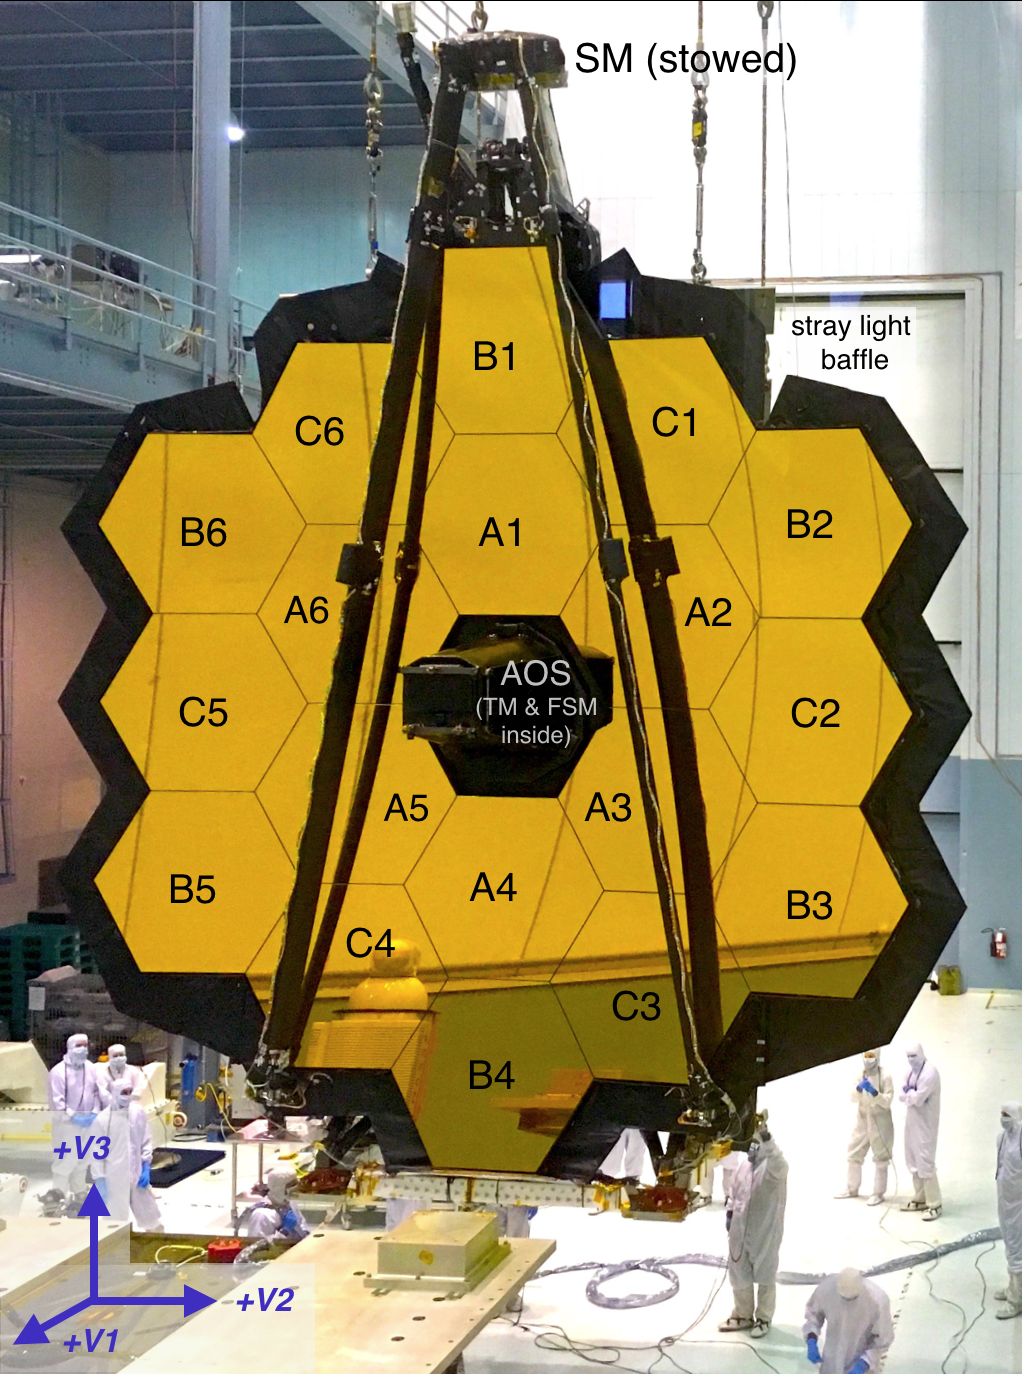
\includegraphics[width=0.9\linewidth]{images/jwst_ote_reflectors.png}
    \caption{JWST: OTE Reflectors setup and reference \cite{JWST_Telescope_Optics}}
    \label{fig:jwst_ote_reflectors}
\end{figure}

Each segment of the mirror has at most $\sim 25 nm$ error, which is only $\frac{1}{15.2}$ of $380nm$, the bottom of the visible light spectrum. Each segment also has 6 actuators attached to the back to allow small adjustments of the spatial angle of $\sim 10nm$ and a seventh actuator to correct any problems created during manufacturing and travel to match the focal length of all 18 segments.

The secondary mirror is a convex circular mirror that focuses light towards the tertiary mirror. Both the primary and secondary mirror create a pseudo-cassegrain telescope, which flips the incoming image before it hits the next mirror.

The tertiary mirror is a static concave aspheric mirror reflecting light back towards the front onto the FSM and cancelling aberrations.

The last mirror before the light enters ISIM is the already mentioned adjustable flat fine steering mirror. Its job is to make slight adjustments during the observations to stabilise the image.

All of these mirrors also have the same maximum error of $\sim 25nm$ as the primary mirror. The complete optical system diagram can be seen in figure \ref{fig:jwst_ote_diagram}.

\begin{figure}[h]
    \centering
    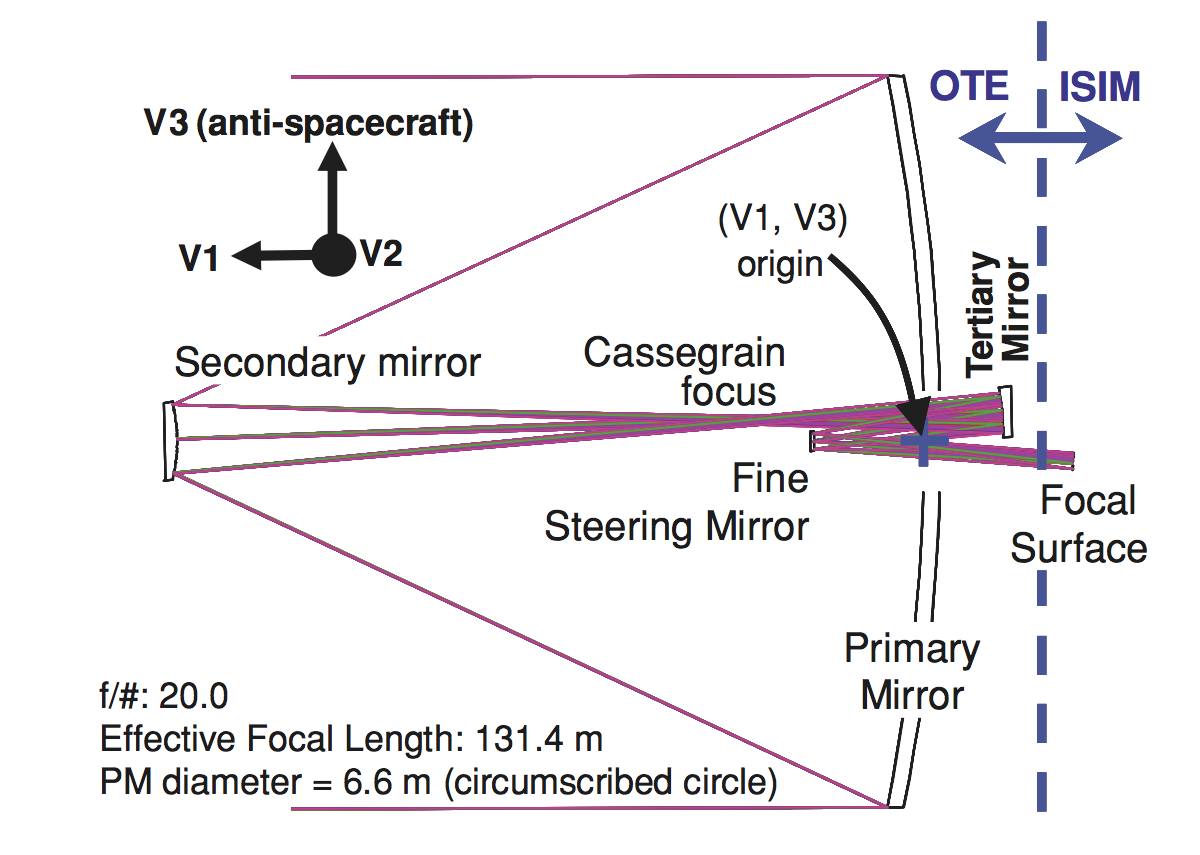
\includegraphics[width=0.9\linewidth]{images/jwst_ote_diagram.png}
    \caption{JWST: OTE Light Reflection Diagram \cite{JWST_Telescope_Optics}}
    \label{fig:jwst_ote_diagram}
\end{figure}

This setup can create much better results than the one found onboard HST OTA \ref{subsec:hst_ota}, but is also much more complex during construction, setup, and observation. The reason for the number of adjustable parts within the OTE compared to the static approach of OTA is the inability of servicing. The HST is within low-Earth orbit, and regular maintenance missions were possible, which came in handy during the initial issues the HST had that were fixed with corrective optics. The JWST is within the L2 orbit and any maintenance or upgrade missions, at least for the foreseeable future, are impossible, and so any adjustments and fixes must be done remotely.

Another thing to keep in mind regarding the OTE is that an expected side-effect of the hexagonal reflector setup is that the observations, especially those done on point light sources, will have artefacts of the hexagonal setup and reflector edges. This is best seen in comparison between images from the HST and the JWST in figure \ref{fig:comparing_jwst_hst}, where a distinct shape around stars looks like the intersection edges of the hexagonal segments.

\subsection{Integrated Science Instrument Module}

The ISIM contains 4 multi-purpose instruments (each instrument has 4+ modes), the Fine Guidance Sensor and the Command and Data Handling subsystem, which handles many functionalities like event-driven observations, target acquisitions, etc \cite{JWST_ISIM}. The four instruments on-board are:

\begin{itemize}
    \item Mid Infrared Instrument (MIRI)
    \item Near Infrared Camera (NIRCam)
    \item Near Infrared Imager and Slitless Spectrograph (NIRISS)
    \item Near Infrared Spectrograph (NIRSpec)
\end{itemize}

As can be seen, most of the instruments work within the infra-red light spectrum, which is used to counter light dispersion that occurs over a long distance of space. Visible light coming in from outer space gets slowly longer and thus shifts into infra-red light, also called a \textit{redshift}. The JWST and other telescopes handle this by capturing light in IR and then processing the data back into a visible light equivalent, thus giving us images such as seen in figure \ref{fig:comparing_jwst_hst}. This is also the reason for the low operating temperature and shielding from any IR that might come from the sun or the rest of the telescope.

Lastly, each instrument within the layout of the focal plane has both an offset and angle offset. These offsets can be seen in figure \ref{fig:jswt_instrument_focal_plane}, which also shows the size of each sensor area and the layout of sensors within an instrument.

\begin{figure}[h]
    \centering
    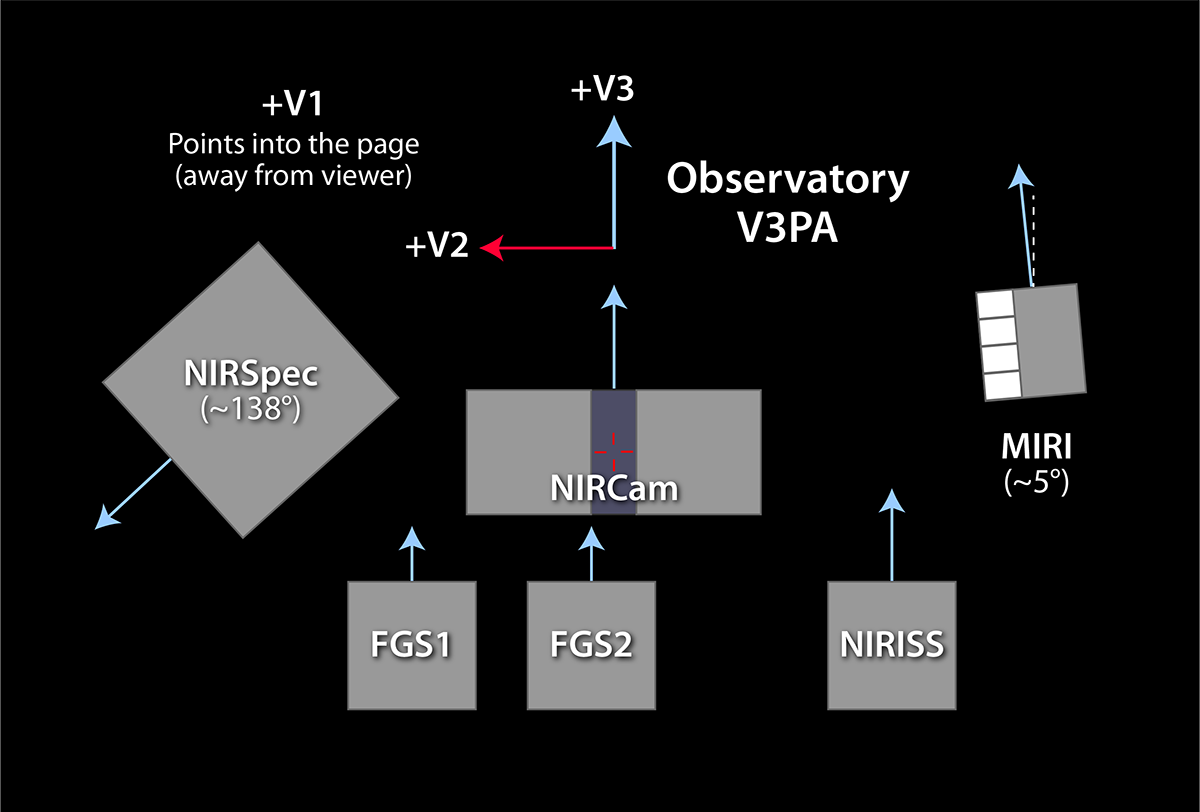
\includegraphics[width=0.95\linewidth]{images/jwst_focal_plane_instruments.png}
    \caption{JWST: The layout of instruments in the focal plane.}
    \label{fig:jswt_instrument_focal_plane}
\end{figure} 

\begin{figure*}
    \centering
    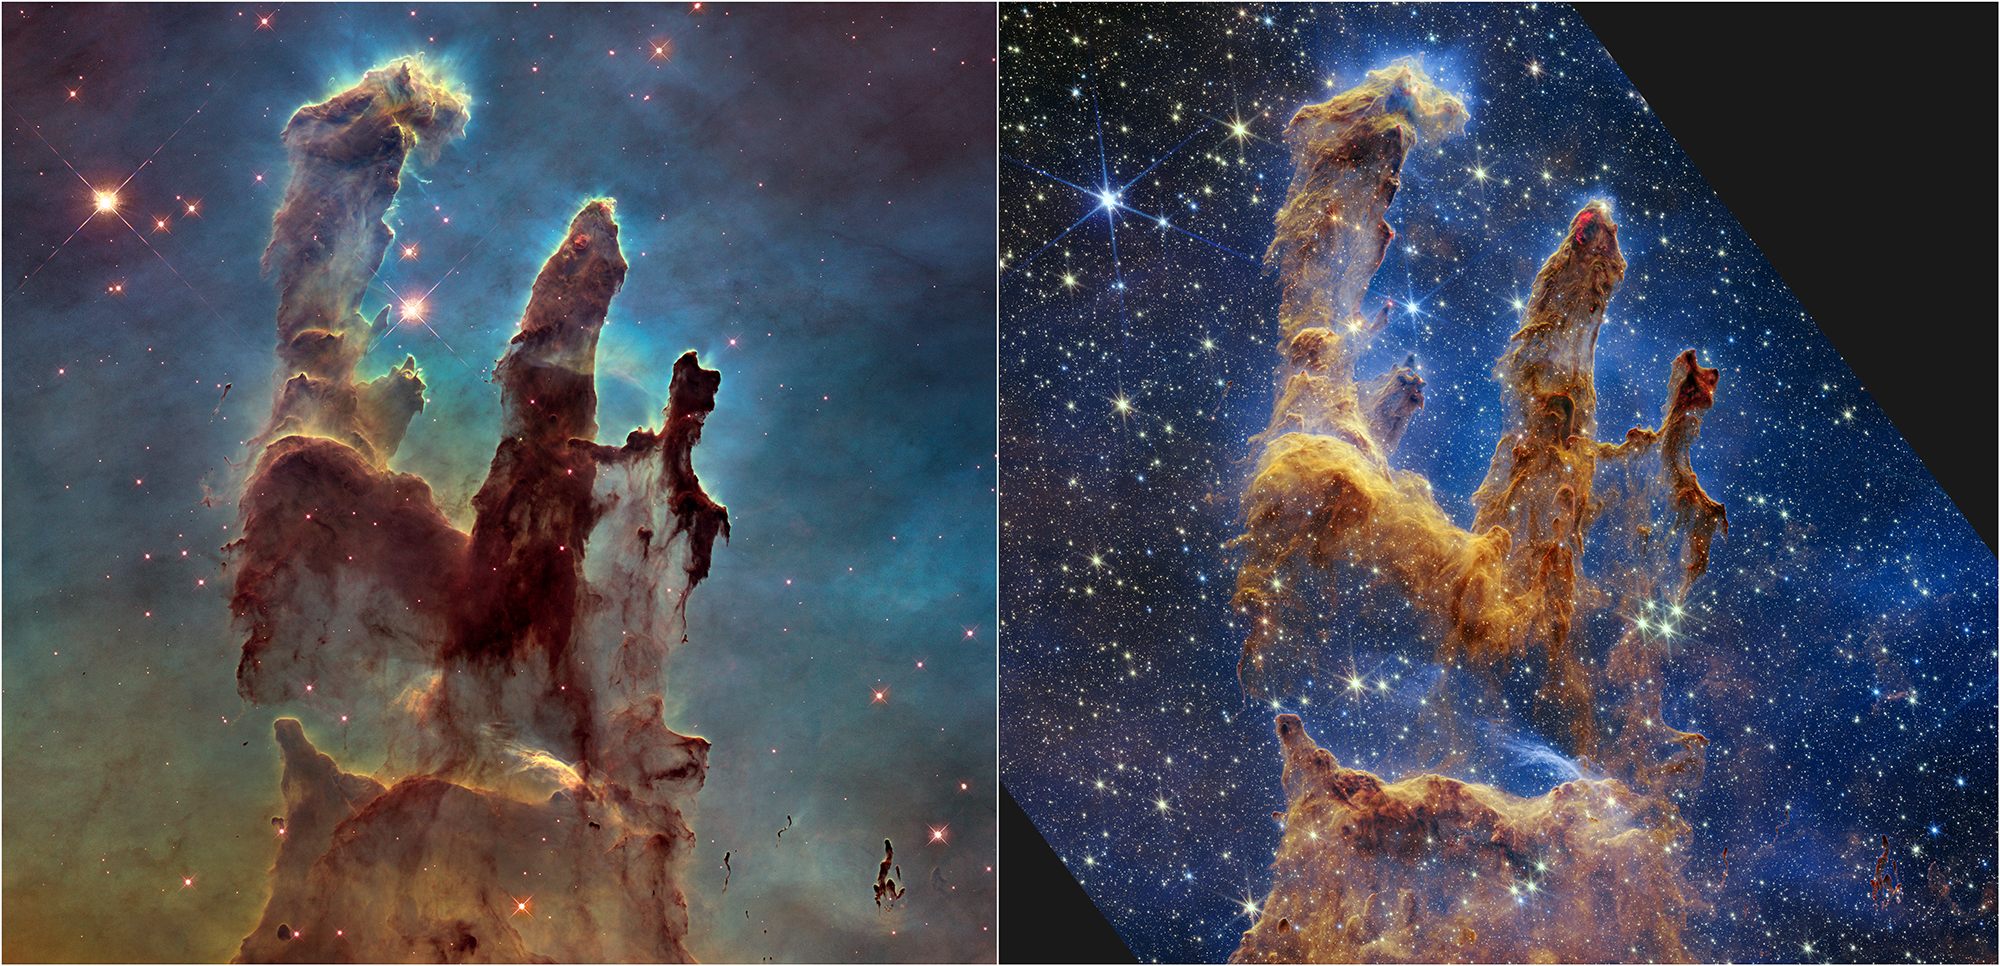
\includegraphics[width=0.9\linewidth]{images/jwst_comparing_hst.png}
    \caption{Comparing images between HST (left) and JWST (right)  \cite{Roshni_Printer_2026_edu}}
    \label{fig:comparing_jwst_hst}
\end{figure*} 

\subsection{Mid Infrared Instrument}

The MIRI instrument observes light within the $\sim 5$ to $28 \unit{\micro\meter}$ range through 4 separate modes. It is designed as a multi-purpose instrument that handles several functionalities, and as can be seen in figure \ref{fig:jswt_instrument_focal_plane}, it contains several differently sized sensors, each handling a different mode. The four modes include:

\begin{table}[h]
    \centering
    \begin{tabular}{lr}
        \textbf{Mode} & \textbf{Wavelength ($\unit{\micro\meter}$)}  \\
        Imaging & $\sim5\text{-}26$ \\
        Coronagraphic Imaging & $\sim10\text{-}23$ \\
        Low-Res Spectroscopy & $\sim5\text{-}14$ \\
        Medium-Res Spectroscopy & $\sim5\text{-}28$ \\
    \end{tabular}
    \caption{JWST: MIRI Modes \cite{JWST_MIRI}}
    \label{tab:jwst_ote_information}
\end{table}

\subsection{Near Infrared Camera}

Like the MIRI, the NIRCam is a multi-purpose instrument that works in much smaller wavelengths (near infra-red) of $0.6$ to $5.0 \unit{\micro\meter}$. It also has 4 modes, which are:

\begin{table}[h]
    \centering
    \begin{tabular}{lr}
        \textbf{Mode} & \textbf{Wavelength ($\unit{\micro\meter}$)}  \\
        Imaging & $0.6 \text{-} 2.3 \& 2.4 \text{-} 5.0$ \\
        Coronography & $1.8 \text{-} 2.2, 2.8 \text{-} 5.0$ \\
        Wide Field Slitless Spectroscopy & $0.6 \text{-} 2.3, 2.4 \text{-} 5.0$ \\
        Time-Series Monitoring & $0.6 \text{-} 2.3, 2.4 \text{-} 5.0$ \\
    \end{tabular}
    \caption{JWST: NIRCam Modes \cite{JWST_NIRCam}}
    \label{tab:jwst_ote_information}
\end{table}

The observations are split into two sections (lightpaths) depending on the wavelength. The incoming light is split by dichroic beam splitter (optionally going through a coronagraphic occulting mask) into shorter ($0.6 \text{-} 2.3 \unit{\micro\meter}$) and long ($2.4 \text{-} 5 \unit{\micro\meter}$) wavelengths. Each path uses a combination of two wheel assemblies: Pupil and Filter to adjust the observations.

The NIRCam overall uses 10 Teledyne HgCdTe H2RG detectors within special arrays. Eight of these detectors are assembled into two square groups of four with $4\text{-}5''$ distances within the group and $44''$ distance between the groups. The remaining two detectors are nearly the same size as one group, placed within the same FOV place as the groups, and are used for longer wavelength detection simultaneously as the group detection.

\subsection{Near Infrared Imager and Slitless Spectrograph}

Unlike the previous 2 instruments, NIRISS only has one sensor with the FOV $133''$, but, just like the previous instruments, it has 4 modes:

\begin{table}[h]
    \centering
    \begin{tabular}{lr}
        \textbf{Mode} & \textbf{Wavelength ($\unit{\micro\meter}$)}  \\
        Imaging & $0.8 \text{-} 5.0$ \\
        Wide Field Sl Spectroscopy & $0.8 \text{-} 2.2$ \\
        Single Object Sl Spectroscopy & $0.6 \text{-} 2.8$ \\
        Aperture Mask Interferometry  & $2.8 \text{-} 4.8$ \\
    \end{tabular}
    \caption{JWST: NIRCam Modes \cite{JWST_NIRISS}}
    \label{tab:jwst_ote_information}
\end{table}

Switching between these modes and other minor adjustments are done through a pair of selection wheel assemblies: Pupil wheel and Filter wheel.

\subsection{Near Infrared Spectrograph}

The last instrument NIRSpec, as its name suggests, provides near-IR spectroscopy from $0.6\text{-}5.3 \unit{\micro\meter}$ within a $3.4' \times 3.6'$ FOV. It uses a micro-shutter assembly with integral field units and fixed slits in its design. The NIRSpec also has 4 obervation modes:

\begin{table}[h]
    \centering
    \begin{tabular}{lr}
        \textbf{Mode} & \textbf{Apert. or Slit Size ($''$)}  \\
        MSA Spectroscopy & $0.20 \times 0.46$ \\
        IFU Spectroscopy & $3.0 \times 3.0$ \\
        Fixed Slit Spectroscopy & $0.2 \times 3.2, \dots$ \\
        Bright Object Time Series   & $1.6 \times 1.6$ \\
    \end{tabular}
    \caption{JWST: NIRCam Modes \cite{JWST_NIRSpec}}
    \label{tab:jwst_ote_information}
\end{table}

To select each mode or adjust observations the NIRSpec uses two wheel assemblies: Filter and Grating. The detectors are two $5.3 \unit{\micro\meter}$ cut-off HgCdTe arrays, each having $2048 \times 2048$ pixel resolution.

\subsection{Fine Guidance Sensor}

Unlike with the FGS onboard the HST, the FGS onboard the JWST contains only one near-IR sensor (camera), but just like on the HST it is used for adjustments and stabilisation of the optical axis using reference stars during observations. 

It uses two channels: Guider1 and Guider2, which it uses for its two main functions. The first is to acquire and observe predetermined guide stars, which are sent to the Attitude Control Subsystem for attitude determination. The second function sends pointing data to the subsystem for attitude stabilisation for both fixed point and moving targets during exposure.

\section{Visualization}

There are several possible visualisation options within this project, of which I have chosen a more broad one. Instead of focusing on one or two instruments, I wanted to create a visualisation of the entire telescopes within orbit coupled with additional information about the optics and instruments. In other words, a more broad educational visualisation than a specific scientific one.

For the implementation, I have chosen for myself a familiar Godot 4.6 platform, which is an open-source game engine. This means that without giving up much freedom, I get a full rendering pipeline, objects, scripting, etc, without having to worry about low level implementation. The engine approach also allows me to create stable exports for multiple platforms, especially Windows, which is the project target.

The initial idea was to visualise both telescopes in their respective orbits, but that idea was scrapped for a more static approach due to both runtime requirements, complications, and disorientation. This also allows for reference objects to be placed next to the telescopes for a better understanding of the scale.

The visualisation now offers models for both telescopes, information about them and their instruments, cross-section of the HST, and the option to see the wavelength ranges for each telescope/instrument. The controls are fully realised by mouse clicks/movement. The information and functionality window can be closed, resized, and moved.

Models for both telescopes are sourced from the official NASA sites, and additional reference scale models are sourced from the internet for free.